\section{Modelos económicos}

Un modelo económico es una abstracción del mundo real. Consiste en un conjunto de ecuaciones que representan, de manera simplificada, 
las relaciones entre variables con el fin de describir y analizar la estructura y el comportamiento de un fenómeno, en este caso económico.



\subsection{Elementos de un modelo matemático}

\subsubsection{Variables, constantes y parámetros}

Una \textit{variable} es algo cuya magnitud puede cambiar. En economía, las variables más utilizadas suelen ser el
precio, ganancia, costo, ingreso nacional, consumo, inversión, importaciones y exportaciones.

Hay dos tipos de variables
\begin{itemize}
    \item Endogenas: aquellas cuyos \textit{valores de solución} se originan desde dentro, desde el mismo modelo.
    Por ejemplo el nivel de producción maximización ganancia.
    \item Exógenas: aquellas determinadas por fuerzas externas al modelo
\end{itemize}

Una \textit{constante} es una magnitud que \textbf{no} cambia. 

Una \textit{constante parametrica o parametro} es una constante a la cual se le puede asignar un valor, es decir 
es una constante que es variable.

\subsubsection{Ecuaciones e identidades}

En la economía hay 3 tipos de ecuaciones
\begin{itemize}
    \item Ecuaciones definicionales: establece una identidad\footnote{Identidad es una definición, una verdad absoluta. Por ejemplo \(1 \equiv 1\)} 
    entre 2 expresiones que tienen \textit{el mismo significado}. Para una ecuación definicional se utiliza el simbolo \equiv.
    Por ejemplo
    \[
    \pi \equiv R - C
    \]
    Donde \(R\) es el exeso de ingreso total, \(C\) es el costo total y \(\pi\) es el la ganancia total 
    \item Ecuaciones de comportamiento: especifíca como se comporta una variable en respuesta a cambios en otras variables. Por ejemplo 
    cuanto gasta la gente en función de sus ingresos.
    \[
    C = \alpha + bY
    \]
    Donde \(C\) es el consumo total, \(\alpha\) el consumo autónomo (Lo que la gente gasta incluso si no tiene ingresos), \(b\) la propersión a consumir e \(Y\) el ingreso nacional
    \item Ecuaciones condicionales: deben satisfacer un requerimiento. Por ejemplo la condición de equilibro como requisito en el caso de
    \begin{gather*}
        Q_d = Q_s \quad \text{Cantidad demandada} = \text{Cantidad suministrada} \\ S = I \quad \text{Ahorro previsto} = \text{inversión prevista}
    \end{gather*}
\end{itemize} 




\subsection{Sistema de numeros reales}

Los números \textit{enteros} son los de uso común, como: 1, 2, 3... Estos pueden ser negativos.
Los números enteros forman una fracción, como: \(\frac{2}{3}\), es decir los enteros constituyen el \textit{conjunto de fracciones}.

El conjunto de enteros y el conjunto de fracciones forman el conjunto de \textit{números racionales}, el número racional es aquel que se puede expresar 
con un decimal, que puede ser finito (0.25) o periódico (0.3333...).

Los \textit{números irracionales} son aquellos que no se pueden expresar como razon de un par de enteros, como por ejemplo: \(\sqrt{2} = 1.4142\dots\), que es 
un decimal no periódico, no finito. Otro ejemplo es \pi.

Los \textit{números reales} son aquellos que pueden tomar cualquier valor numérico. En la recta de los números racionales existen puntos que no están
representados, al igual que ocurre en la recta de los números irracionales. Los números reales integran ambos conjuntos los racionales y los irracionales, 
formando una recta numérica continua que completa las carencias de cada uno de ellos, por esta razón se dice que la recta de los números reales es continua.
 Se ejemplifica esto en la figura \ref{fig_numeros_reales} y \ref{fig_recta_numeros_reales}.

\begin{figure}[ht]
    \centering
    \includegraphics[width=0.7\textwidth]{./media/chapter/01_introducation/numeros_reales.png}
    \caption{El conjunto de números reales está formado por los conjuntos de números racionales e irracionales.}
    \label{fig_numeros_reales}
\end{figure}

\begin{figure}[ht]
    \centering
    \includegraphics[width=0.7\textwidth]{./media/chapter/01_introducation/recta_numeros_reales.png}
    \caption{La recta de números reales es una línea continua, ya que \textit{no} contiene números faltantes.}
    \label{fig_recta_numeros_reales}
\end{figure}




\subsection{Concepto de conjuntos}

\subsubsection{Notación de conjuntos}

Un \textit{conjunto} es una colección de objetos distintos, los cuales pueden ser un grupo de números, personas, etc. 
Los objetos que forman parte de conjunto se los llama \textit{elementos} del conjunto.

Un conjunto se puede escribir por
\begin{itemize}
    \item Enumeración. Por ejemplo \(\quad S = \{ 1,\, 2,\, 3 \}\) 
    \item Descripción. Por ejemplo \(\quad l = \{ x ~|~ x\text{ es un número entero positivo} \}\)
\end{itemize}

En el ejemplo del conjunto descriptivo \(l\) es el conjunto de todos los números \(x\), tales \(|\) que \(x\) es un entero positivo.\footnote{El simbolo \(|\) significa ``tal que''.}
Todo conjunto se encierra con \(\{ \}\), y en el caso del descriptivo, \textit{se utiliza} \(|\) o \(:\) \textit{para separar el símbolo de designación
del elemento de la descripción de estos}. Por ejemplo, un conjunto descriptivo de números \(\mathbb{R}\) (reales) mayores que 2 pero menores que 5
se puede expresar como \(J = \{ x ~|~ 2 < x < 5 \}\)

En el primer punto, \(S\) es un \emph{conjunto finito}. Mientras que en el segundo punto, \(l\) es un \emph{conjunto infinito}.
Los conjuntos finitos \textit{siempre} son \emph{numerables}, mientras que los conjuntos infinitos pueden o no ser \emph{numerables}.
\(l\) es un conjunto infinito numerable, mientras que \(J\) es un conjunto infinito inumerable, ya que \(l\) se basa en números
enteros, mientras que \(J\), se basa en números reales.

\paragraph{Pertenencia \in }

Se dice que un elemento pertence a un conjunto cuando este elemento se encuentra en el mismo, quizas suena confuso, veamoslo con un ejemplo
\[
2 ~ \in ~ S \qquad 3 ~ \in ~ S
\]
En el ejemplo estamos diciendo que tanto \(2 ~\text{como}~ 3\) pertenecen \(\in\) a \(S\)

Cuando queremos decir que un elemento \textbf{no} pertence a un conjunto utilizamos \(\notin\). Por ejemplo
\[
8 ~ \notin ~ S
\]
\(8\) No pertenece a \(S\), ya que si recordamos \(S = \{ 1,\, 2,\, 3 \}\), no incluye ningún elemento más que \(\{ 1,\, 2,\, 3\}\)

En el caso de \(l\), recordemos que \(l = \{ x ~|~ x\text{ es un número entero positivo} \}\), podemos decir que \(x ~ \in ~ \mathbb{R} \), que quiere
decir que la variable x puede ser cualquier número que exista en la recta real.


\subsubsection{Relaciones entre conjuntos}

Dos conjuntos son iguales cuando contienen elementos idénticos. Por ejemplo 
\[
S_1 = \{2 ,\,  7 ,\,  \alpha ,\,  f\} \qquad = \qquad S_2 = \{2 ,\,  \alpha ,\,  7 ,\,  f\}
\]

Como se puede ver el orden de aparición de los elementos en un conjunto es de poca importancia. Sin embargo si se encuentra un solo elemento
diferente en uno de los conjuntos, esos conjuntos no son iguales.

Un conjunto puede ser un \emph{subconjunto} de otro conjunto. Por ejemplo
\[
S = \{2 ,\,  3 ,\,  5 ,\,  7 ,\,  9\} \qquad \text{y} \qquad T = \{3 ,\,  7 \}
\]
Donde \(T\) es un subconjunto de \(S\), ya que todo elemento de \(T\) es un elemento de \(S\).
Es decir \(T\) es un subconjunto de \(S\), donde si \(x ~\in~ T\) implica que \(x ~\in~ S\). 

Simbolicamente podemos decir que un conjunto esta \emph{contenido en otro conjunto} con \(\subset\). 
Y podemos decir que un conjunto \emph{incluye} a otro conjunto con \(\supset \). Es decir, basandonos en el ejemplo anterior de
\(T\) y \(S\)
\[
T ~\subset~ S \qquad y \qquad S~ \supset ~T 
\]

Dos conjuntos pueden ser subconjuntos entre sí, lo cual significa que ambos conjuntos son iguales. Es decir si 
\(S_1 ~=~ S_2\) \quad \(S_1 ~\subset~ S_2~\) y \(~S_2 ~\subset~ S_1\).

A partir del subconjunto \(S = \{1,\, 3,\, 5,\, 7,\, 9\}\) se pueden formar \(2^5 = 32\) subconjuntos, ya que un subconjunto
puede ser un elemento del conjunto o un conjunto de elementos.

Todo subconjunto que \textit{no} contiene a \textit{todos} los elementos de \(S\) se llama \emph{subconjunto propio} de \(S\). 
El conjunto de los \(5\) elementos del conjunto \(S\) es un subconjunto de \(S\), pero no es un subconjunto propio. 
Es decir, el caso límite en el que un subconjunto deja de ser propio, es cuando el mismo es igual al conjunto original, ya que ese es 
el subconjunto más grande posible\footnote{Es como decir que el límite de "una parte de la pizza" es "la pizza entera".}. 

El subconjunto más pequeño posible (el otro caso límite) es un conjunto de \(S\) que \textit{no} contiene ningún elemento.
Este conjunto se conoce como \textit{conjunto nulo} o \textit{conjunto vacío} y se simboliza con \(\varnothing\) o \(\{\}\).
Se considera al conjunto nulo de \(S\) como un subconjunto ya que si \(\varnothing\) no fuera un subconjunto de \(S\) significaria que \(\varnothing\) 
deberia contener al menos un elemento tal que \(x\) \(\notin\) \(S\). Pero como \(\varnothing\) no tiene ningun elemento en absolunto, no podemos
decir que \(\varnothing \not\subset S\).
\textit{Todo} conjunto incluye al \textit{conjunto nulo}.

Sabiendo los casos limites explicados anteriormente, podemos afirmar que el conjunto \(S\) puede formar \(32\) elementos. Veamoslo con otro caso,
donde \(S = \{1 ,\,  2 ,\, 3\}\). Si quisieramos saber cuantos subconjuntos se pueden formar del conjunto \(S\) 
podemos armar una tabla como se muestra en el cuadro \ref{subconjuntos_del_conjunto_S}.
\begin{table}[h]
    \centering
    \begin{tabular}{|c|c|}
    \hline
    Subconjunto & elementos  \\
    \hline
    1 & \{1\} \\
    2 & \{2\} \\
    3 & \{3\} \\
    4 & \{1 ,\,  2\} \\
    5 & \{1 ,\,  3\} \\
    6 & \{2 ,\,  3\} \\
    7 & \{1 ,\,  2 ,\,  3\} \\
    8 & \varnothing \\
    \hline
    \end{tabular}
    \caption{De \(S\) se forman \(2^3 = 8\) subconjuntos}
    \label{subconjuntos_del_conjunto_S}
\end{table}

Dos conjuntos pueden no tener elementos en común en absoluto, en este caso se dice que los conjuntos son \textit{disjuntos}.
Si dos conjuntos tienen \textit{algunos} elementos en común, pero algunos propios de cada uno, se dice que no son iguales ni disjuntos.



\subsubsection{Operaciones con conjuntos}

Los conjuntos se pueden \emph{unir}, \emph{intersectar} y \emph{complementar}.

La \emph{unión} de dos conjunto, \(A\) y \(B\) forman un nuevo conjunto que contiene los elementos que pertenecen a \(A\) o \(B\),
o a \(A\) y \(B\). La unión se simboliza como \(A ~\cup ~ B\).

Si \(A = \{3 ,\,  5 ,\,  7 \}\) y \(B = \{2 ,\,  3 ,\,  4 ,\,  8\}\) la union de \(A\) y \(B\) seria
\[
A ~\cup~ B = \{2 ,\,  3 ,\,  4 ,\,  5 ,\,  7 ,\,  8\}
\]

En este caso \(A\) y \(B\) no son iguales ni disjuntos y ninguno es subconjunto del otro.

La \emph{intersección} de dos conjuntos \(A\) y \(B\) es un nuevo conjunto que contiene a los elementos que pertenencen \textit{tanto a \(A\) como a \(B\)}.
La intersección se simboliza como \(A ~\cap ~ B\)
Utilizando los datos de \(A\) y \(B\), la intersección de \(A\) y \(B\) es \(\{3\}\), es decir 
\[
A ~\cap~ B = \{3\}
\]

En el caso que \(A\) y \(B\) \textit{no} tengan ningun elemento igual, \(A ~\cap~ B = \varnothing\). El conjunto \(A\) y el conjunto
\(B\) son disjuntos, por lo tanto su itersección es el conjunto nulo \varnothing. Ya que ningún elemento es común.

Entonces, decimos que:
\begin{itemize}
    \item Intersección \qquad \(A ~\cap~ B = \{x~|~x \in A \quad \textbf{y} \quad x \in B\}\)
    \item Unión \qquad \(A ~\cup~ B = \{x~|~x \in A \quad \textbf{o} \quad x \in B\}\)
\end{itemize}

El \emph{complemento de un conjunto}. Para entender que es el complemento de un conjunto se tiene que entender el concepto de conjunto universal.

Un \textit{conjunto universal} es un conjunto de \(n\) números que representan el universo de dicho conjunto, supongamos \(U = \{1 ,\,  2 ,\, 3\}\), 
\(U\) representa el universo, vease en la figura \ref{fig_operacion_de_conjuntos} donde \(U = A+\tilde{A} \), es decir, el universo es igual a la sumatoria
del conjunto \(A\) y el conjunto \(\tilde{A}\), donde \(A = \{1 ,\, 2\}\) y \(\tilde{A} = 3\). Entonces el complemento del conjunto \(A\) es \(\tilde{A}\),
ya que con este se contienen todos los elementos del universo, es decir, la unión de \(A \cup \tilde{A} = U = \{1 ,\,  2 ,\, 3\}\).

Dicho de otra manera
\[
\tilde{A} = \{x~|~x \in U \quad \text{y} \quad x \notin A\}
\]
El complemento se simboliza con \(\tilde{\phantom{a}}\) y significa \textit{no}.

\begin{figure}[ht]
    \centering
    \includegraphics[width=0.7\textwidth]{./media/chapter/01_introducation/operacion_de_conjuntos.jpg}
    \caption{Diagrama de Venn}
    \label{fig_operacion_de_conjuntos}
\end{figure}

El universo tiene un complemento, este es el conjunto nulo, es decir \(\tilde{U} = \varnothing\).



\subsubsection{Leyes de operaciones con conjuntos}

\paragraph{Ley conmutativa}
Se utiliza para uniones o intersecciones, donde el orden de los elementos no altera el resultado de la \textit{unión} o 
\textit{intersección} del conjunto, es decir 
\[
A ~\cup ~ B = B ~\cup~ A
\]
unir los elementos de \(A\) y \(B\) da el mismo resultado que unir los de \(B\) y \(A\).

En el caso de la intersección los elementos que comparten \(A\) con \(B\) son exactamente los mismos que comparte \(B\) con \(A\),
simbolicamente
\[
A ~\cap ~ B = B ~\cap~ A
\]

\paragraph{Ley asociativa}
La unión o intersección de 3 o más conjuntos, supongamos \(A\), \(B\), \(C\) primero unimos o intersectamos dos conjuntos, para luego
unir o intersectar con el conjunto restante
\begin{gather*}
    A ~\cup ~ (B ~\cup~ C) = (A~\cup~B) ~\cup~ C \\
    A ~\cap ~ (B ~\cap~ C) = (A~\cap~B) ~\cap~ C
\end{gather*}

Lo cual se puede apreciar en la figura \ref{fig_ley_asociativa_conjuntos}. El orden en el cual se eligan los conjuntos es intrascendente.
\begin{figure}[ht]
    \centering
    \includegraphics[width=0.7\textwidth]{./media/chapter/01_introducation/Leyes_de_conjuntos.jpg}
    \caption{Representacion grafica de la ley asociativa de \(A\), \(B\), \(C\)}
    \label{fig_ley_asociativa_conjuntos}
\end{figure}

\paragraph{Ley distributiva}
Involucra utilizar tanto la unión y la intersección de manera simultanea. Es similar a distribuir de manera algeibraica.

La \textit{distribución de la unión sobre la intersección}, es aquella en la cual se quiere unir un conjunto, supongamos \(A\) con
la intersección de \(B\) y \(C\), que seria lo mismo que unir \(A\) con \(B\) y \(A\) con \(C\) para luego ver donde intersectan, es decir
\[
A \cup (B \cap C) = (A \cup B) \cap (A \cup C)
\]

La \textit{distribución de la intersección sobre la unión}, es cuando se quiere intersectar el conjunto, supongamos \(A\) con la unión de \(B\) 
y \(C\), lo cual sería lo mismo que intersectar \(A\) con \(B\) y \(A\) con \(C\) para luego unir el resultado, es decir
\[
A \cap (B \cup C) = (A \cap B) \cup (A \cap C)
\]

Vamos a comprobar y verificar la ley distributiva, dado \(A = \{4 ,\,  5 \}\), \(B = \{3 ,\,  6 ,\, 7\}\) y 
\(C = \{2 ,\,  3 \}\), basandonos en la distribución de la unión sobre la intersección, donde 
\[
A \cup (B \cap C) = (A \cup B) \cap (A \cup C)
\]
Para que la operación se vea más prolija, dividamosla en 2 partes 
\begin{itemize}
    \item \(A \cup (B \cap C)\) remplazamos: \(\{4 ,\,  5 \} ~\cup~ \{3\} = \{3 ,\,  4 ,\, 5\}\) 
    \item \((A \cup B) \cap (A \cup C)\) remplazamos: \(\{3 ,\,  4 ,\, 5 ,\,  6 ,\,  7 \} ~\cap~ \{2 ,\,  3 ,\, 4 ,\,  5\} = 
    \{3 ,\,  4 ,\, 5\} \)
\end{itemize}

Basandonos en la distribución de la intersección sobre la unión, donde
\[
A \cap (B \cup C) = (A \cap B) \cup (A \cap C)
\]
Al igual que en el caso anterior vamos a dividir la operación para que sea más prolija
\begin{itemize}
    \item \(A \cap (B \cup C)\) remplazamos: \(\{4 ,\,  5 \} ~\cap~ \{2 ,\,  3 ,\,  6 ,\, 7\} = \varnothing\) 
    \item \((A \cap B) \cup (A \cap C)\) remplazamos: \(\{\varnothing\} ~\cup~ \{\varnothing\} = \varnothing\)
\end{itemize}

Habiendo concluido nuestras operaciones, podemos confirmar que el resultado para este caso es el mismo, por lo tanto es una ley valida.



\begin{tcolorbox}[
  title=Ejercicios de conjuntos,
  breakable,
  colback=gray!5,
  colframe=gray!60
]
\begin{enumerate}
  \item Escribir en notación de conjuntos:
  \begin{itemize}
    \item El conjunto de números reales mayores que 34. 

    Respuesta: \(A = \{x \in \mathbb{R}~|~ x > 34\}\)
    \item El conjunto de números reales mayores que 8 pero menores que 65
    
    Respuesta: \(B = \{x ~|~ x > 8 ~\text{y}~ x < 65 \}\)
  \end{itemize}
  \item Dado los conjuntos \(S_1 = \{2 ,\,  4 ,\, 6\}\), \(S_2 = \{7 ,\,  2 ,\, 6\}\), 
  \(S_3 = \{4 ,\,  2 ,\, 6\}\) y \(S_4 = \{2 ,\,  4\}\) responda: 
    \begin{itemize}
        \item \(S_1 = S_3\)  Respuesta: Verdadero
        \item \(S_1 = \mathbb{R}\)  Respuesta: Falso. \(S_1\) es un subconjunto de \(\mathbb{R}\), no es igual.
        \item \(8 \in S_2\)  Respuesta: Falso
        \item \(3 \notin S_2\)  Respuesta: Verdadero
        \item \(4 \notin S_3\)  Respuesta: Falso
        \item \(S_4 \subset \mathbb{R} \)  Respuesta: Verdadero
        \item \(S_1 \supset S_4\)  Respuesta: Falso
        \item \(\varnothing \subset S_2\)  Respuesta: Verdadero
        \item \(S_3 \supset \{1,2\}\)  Respuesta: Falso
    \end{itemize}
  \item En relacion a los conjuntos del problema 2, determinar:
    \begin{itemize}
        \item \(S_1 \cup S_2 \text{ Respuesta: } \{2,4,6,7\}\)
        \item \(S_1 \cup S_2 \text{ Respuesta: } \{2,4,6\}\) 
        \item \(S_2 \cap S_3 \text{ Respuesta: } \{2,6\}\)
        \item \(S_2 \cap S_4 \text{ Respuesta: } \{2\}\)
        \item \(S_4 \cap S_2 \cap S_1 \text{ Respuesta: } \{2\}\)
        \item \(S_3 \cup S_1 \cup S_4 \text{ Respuesta: } \{2,4,6\}\)
    \end{itemize}
   \item ¿Cuál de los encunciados son validos?
    \begin{itemize}
        \item \(A\cup A = A\)  Respuesta: Verdadero
        \item \(A \cap A = A\)  Respuesta: Verdadero
        \item \(A \cup \varnothing = A\)  Respuesta: Verdadero
        \item \(A \cup U = U\)  Respuesta: Verdadero
        \item \(A \cap \varnothing = \varnothing\)  Respuesta: Verdadero
        \item \(A \cap U = A\)  Respuesta: Verdadero
        \item El complemento de \(\tilde{A}\) es \(A\).  Respuesta: Verdadero. 
        
        El complemento del complemento te devuelve al original. Es como decir: "Lo opuesto de (lo opuesto de A)". Si A~ es "lo que no es A", entonces el complemento de eso es "lo que NO no es A", es decir, A.
    \end{itemize}
   \item Enumere los subconjuntos del conjunto \(\{5,6,7\}\)
   
   Respuesta: la cantidad de subconjuntos es \(2^3 = 8\)
   \item Enumere los subconjuntos del conjunto \(\{a,b,c,d\}\)
   
   Respuesta: la cantidad de subconjuntos es \(2^4 = 16\)
\end{enumerate}
\end{tcolorbox}




\subsection{Relaciones y funciones}

\subsubsection{Pares ordenados}

Un par ordenado es aquel en el cual el \textit{orden} de los elementos tiene importancia. Es decir, es aquel donde 
\(A = \{a , b\} \neq  A = \{b , a\}\), excepto sí \(a = b\). Los pares, ternas, cuadruplas ordenadas 
de elementos se pueden llamar en forma colectiva \textit{conjuntos ordenados}, y estos se encierran entre paréntesis 
y no entre llaves, es decir que cuando queremos denotar que un conjunto es ordenado se haria así \(A = (a , b)\)

\begin{ejemplo}[1]
    Los pares ordenados serian utiles para mostrar la edad y el peso de cada estudiante de una clase, se pueden formar 
    pares ordenados de \((edad , peso)\). Podemos ver que \((19 , 127)\) y  \((127 , 19)\) obviamente
    indican cosa diferentes.
\end{ejemplo}

En un plano coordenado rectangular (cartesiano), donde el eje \(x\) y el eje \(y\) se cruzan entre si en un angulo 
recto, dividiendo el plano en cuatro cuadrantes. El plano \(x \, y\) es un conjunto infinitos de puntos, cada
punto representa un par ordenado donde el primer elemento es \(x\) y el segundo elemento es \(y\). Por lo tanto 
un el punto \((4 , 2)\) es \(\neq\) que el punto \(2 , 4\). Esto se puede observar en la figura \ref{cuadro_cartesiano}.

\begin{figure}[!ht]
    \centering
    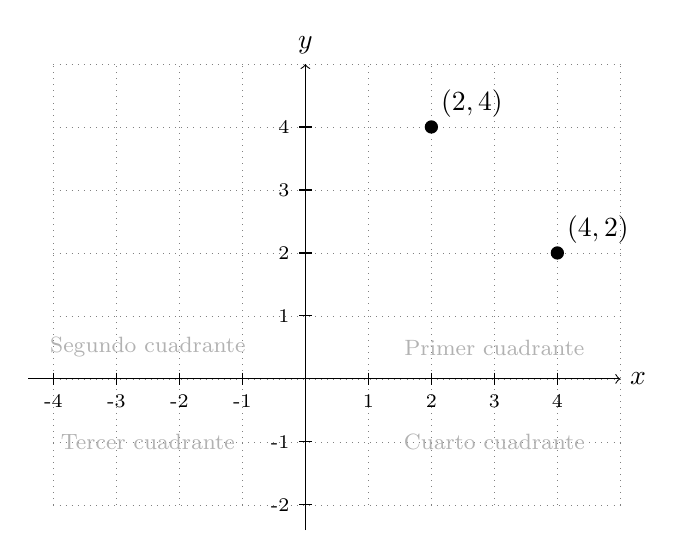
\begin{tikzpicture}[scale=0.8]

        % Cuadrícula suave
        \draw[step=1cm, gray, very thin, dotted] (-4,-2) grid (5,5);
        
        % Ejes
        \draw[->] (-4.4,0) -- (5,0) node[right] {$x$};
        \draw[->] (0,-2.4) -- (0,5) node[above] {$y$};
        
        % Marcas y números eje x
        \foreach \x in {-4,-3,-2,-1,1,2,3,4}
            \draw (\x,0.1) -- (\x,-0.1) node[below] {\scriptsize \x};
        
        % Marcas y números eje y
        \foreach \y in {-2,-1,1,2,3,4}
            \draw (0.1,\y) -- (-0.1,\y) node[left] {\scriptsize \y};
        
        % Punto (4,2)
        \fill (4,2) circle (3pt);
        \node[above right] at (4,2) {$(4,2)$};
        
        % Punto (2,4)
        \fill (2,4) circle (3pt);
        \node[above right] at (2,4) {$(2,4)$};
        
        % Nombre de los cuadrantes
        \node[gray!60] at (3,0.5) {\footnotesize Primer cuadrante};
        \node[gray!60] at (-2.5,0.5) {\footnotesize Segundo cuadrante};
        \node[gray!60] at (-2.5,-1) {\footnotesize Tercer cuadrante};
        \node[gray!60] at (3,-1) {\footnotesize Cuarto cuadrante};
    
    \end{tikzpicture}
    \caption{Cuadro cartesiano con sus respectivos puntos \((4 , 2)\) y \((2 , 4)\)}
    \label{cuadro_cartesiano}
\end{figure}



